%%% Local Variables:
%%% mode: latex
%%% TeX-master: "../report"
%%% End:

\subsection{Installation}
\label{installation}
Get the source:

\quad\code{\$ git clone https://github.com/altschuler/kite.git}

Make sure you have \code{cabal} installed, and then install dependencies:

\quad\code{\$ cabal install}

Build with \code{make}. This will generate an executable in \code{dist/build/kite/}.

\quad\code{\$ make}

To install an executable in \code{\textasciitilde/.cabal/bin}, which will be accessible for your local user:

\quad\code{\$ cabal install}

Make sure that you have the \code{~/.cabal/bin} directory in your \code{PATH}.

Optionally, install globally by putting an executable in \code{/usr/local/bin} (requires root privileges):

\quad\code{\# make install}

For a quick test, try running the KUnit test-suite:

\quad\code{\$ kite tests/kunit/Runner.kite}

The compiler only targets JavaScript, as of now, so make sure you have Node.js installed.

The name of the output file defaults to \code{main}, which executes with \code{node}.

\quad\code{\$ ./main}

You can also run the Haskell test-suite by running:

\quad\code{\$ make test}

\subsection{Kite-mode}
\label{kite-mode}
\lstinputlisting[language=Lisp]{../utils/kite-mode.el}

\subsection{JavaScript runtime}
\label{kt-runtime}
\lstinputlisting[language=Javascript]{../js/kt_runtime.js}

\subsection{Foundation}
\label{foundation}
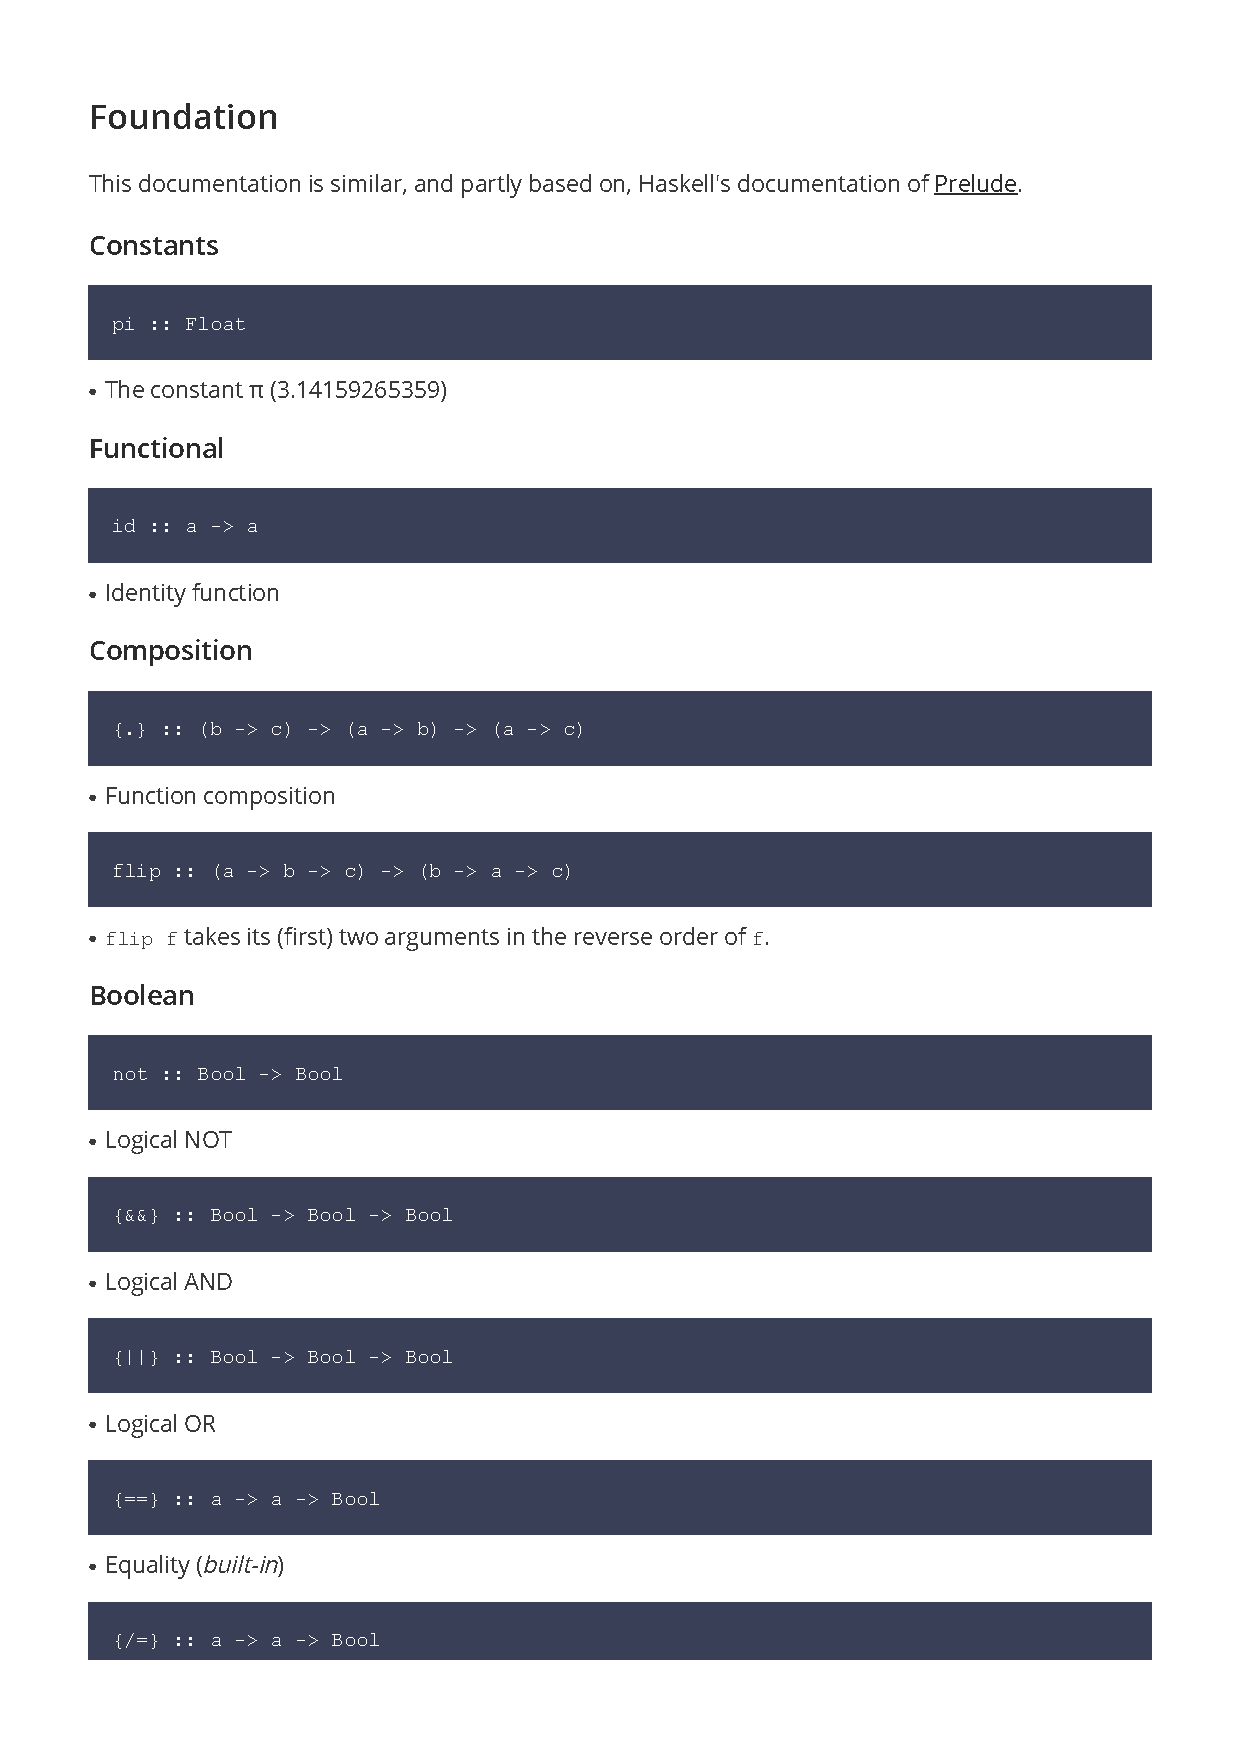
\includepdf[pages=-]{appendices/foundation-doc.pdf}

\subsection{Foundation tests}
\label{sec:foundation-tests}
\verbatiminput{appendices/foundation-tests.txt}
